\documentclass[man, 10pt, floatsintext]{apa7}
\usepackage[spanish, es-nodecimaldot]{babel}
\usepackage{graphfig}
\usepackage{minted}
\setminted{fontsize=\small, baselinestretch=0.9}
\usepackage[utf8]{inputenc}
\usepackage{csquotes}
\usepackage{booktabs}
\usepackage{indentfirst}
\usepackage{setspace}
\usepackage{geometry}
\geometry{margin=2.54cm}
\setlength{\parindent}{1.27cm}

\linespread{2}
\usepackage[style=apa, backend=biber, sortcites=true, doi=true, isbn=true, url=true]{biblatex}
\addbibresource{cap11/bibliografia.bib}

\title{Sistema de Gestión y Seguimiento de Tesis y Proyecto de Grado Para "FICH"}
\shorttitle{}
\author{Marthel Pedro Pozo Solíz \\ Melissa Shanner Nuñez Ardaya \\ Josue Miguel Flores Prado}
\date{\today}

\begin{document}
\hypersetup{pageanchor=false}

\begin{titlepage}

    \begin{center}
        {\fontsize{14pt}{16pt}\selectfont\bfseries\MakeUppercase{Universidad Autónoma Gabriel René Moreno}\par}
        {\fontsize{12pt}{18pt}\selectfont\bfseries\MakeUppercase{Facultad Integral del Chaco}\par}
        {\fontsize{12pt}{18pt}\selectfont\bfseries\MakeUppercase{Carrera Ingeniería Informática y de Sistemas}\par}
        \vspace{1.2cm}
        
\includegraphics[width=0.3\textwidth]{cap0/img/logo2.png}\par
    \end{center}
    {\fontsize{10pt}{16pt}\selectfont\bfseries\MakeUppercase{Sistema de Gestión y Seguimiento de Tesis y Proyectos de Grado para “FICH”}\par}
    \vfill
    {\fontsize{10pt}{14pt}\selectfont\bfseries\MakeUppercase{Integrantes:}\par}
    {\hspace{1cm}\fontsize{10pt}{14pt}\selectfont\bfseries\MakeUppercase{Flores Prado Josue Miguel}\par}
    {\hspace{1cm}\fontsize{10pt}{14pt}\selectfont\bfseries\MakeUppercase{Nuñez Ardaya Melissa Shanner}\par}
    {\hspace{1cm}\fontsize{10pt}{14pt}\selectfont\bfseries\MakeUppercase{Pozo Solíz Marthel Pedro}\par}
    {\fontsize{10pt}{14pt}\selectfont\bfseries\MakeUppercase{Docente:}\par}
    {\hspace{1cm}\fontsize{10pt}{14pt}\selectfont\bfseries\MakeUppercase{Msc. Ing. Evanz Balcazar Veizaga}\par}

    \vfill

    \begin{center}
        {\fontsize{8pt}{14pt}\selectfont\bfseries Camiri, Bolivia \par\today\par}
    \end{center}

\end{titlepage}


\pagenumbering{roman}
\setcounter{page}{2}
\tableofcontents
\listoftables
\listoffigures

\newpage
\pagenumbering{arabic}
\hypersetup{pageanchor=true}
\setcounter{secnumdepth}{3}

\section{Introducción}
\label{sec:introduccion}

% contenido del capítulo

% \input{cap1/subseccion.tex}

\endinput

\newpage
\section{Antecedentes y Justificación}
\label{sec:antecedentes}

\subsection{Antecedentes}

Actualmente en la FICH cada carrera gestiona sus procesos de titulación e investigaciones de forma independiente, sin un sistema unificado. No existe una plataforma institucional ni externa que centralice el seguimiento de tesis y proyectos de grado. En contraste, otras facultades de la UAGRM como Postgrado, Escuela de Ingeniería, Ciencias Jurídicas, Políticas, Sociales y Relaciones Internacionales cuentan con sus propios sistemas, lo que evidencia una carencia en la FICH.

A nivel nacional, \textcite{perales2022repositorios} analizaron el desarrollo de repositorios y revistas científicas de acceso abierto en Bolivia, destacando los avances y rezagos en la comunicación científica universitaria. A nivel internacional, \textcite{leon2012implantacion} presentaron la implantación de un repositorio institucional en la Universidad de Sevilla, basado en tres ejes: recolección, preservación y divulgación. Ambos trabajos sirven como referencia para el diseño del sistema propuesto.

Si bien existen plataformas tecnológicas para la gestión académica, el presente proyecto se enfoca en el desarrollo de una solución a medida para la FICH, por lo que no se adopta ninguna solución existente.

\subsection{Justificación}

El presente proyecto se justifica por sus aportes en tres dimensiones. En el aspecto teórico, contribuye al fortalecimiento de los conceptos de gestión académica, trazabilidad documental y memoria institucional, aplicados al contexto del seguimiento de tesis y proyectos de grado. Desde el punto de vista metodológico, el enfoque de desarrollo basado en casos de uso y la modelización de flujos de trabajo académico constituyen una referencia replicable para proyectos similares en otras unidades de la UAGRM. En el ámbito práctico, el sistema reportará beneficios directos a la FICH al centralizar los procesos de titulación, mejorar la eficiencia operativa, reducir los tiempos de gestión, garantizar el control y respaldo documental, y consolidar la memoria institucional. Asimismo, impactará positivamente en los estudiantes al brindarles un seguimiento claro de su proyecto, en los docentes al facilitar una evaluación sistemática, y en las autoridades al proporcionar datos para la toma de decisiones.

\endinput

\newpage
\section{El Problema}
\label{sec:problema}

\subsection{Situación Problemática}
% Descripción de la situación problemática
En la actualidad se presenta la situación de que la produccion intectual generada en el transcurso del desarrollo de la carrera de cada estudiante, ademas de un desconocimiento de los sistemas para producir el conocimiento que aplica la facultad integral del chaco siguiendo los lineamientos de universidad autonoma Gabriel Rene Moreno


\subsection{Formulación del Problema}
El proceso actual de gestión y seguimiento de tesis y proyectos de grado en la FICH carece de mecanismos sistematizados que garanticen eficiencia en los flujos de trabajo, control sobre el estado de cada proyecto, calidad en la producción intelectual y un respaldo adecuado del conocimiento generado. Actualmente no existe una plataforma unificada que integre el registro de manuscritos, la asignación de tutores y tribunales, el flujo de revisiones y retroalimentación académica, la consulta pública del estado de cada proyecto, la gestión de pagos, ni la generación de reportes y estadísticas. Esta ausencia deriva en retrasos, pérdida de información, falta de trazabilidad y dificultades para que estudiantes, docentes y autoridades den seguimiento oportuno a los procesos de titulación.


\endinput

\newpage
\section{Objetivos}
\label{sec:objetivos}

\subsection{Objetivo General}
Desarrollar un sistema de gestión y seguimiento de tesis y proyectos de grado para la Facultad Integral del Chaco, con el fin de articular la interacción entre tutores y estudiantes y conservar el conocimiento producido en las diferentes carreras de la facultad.

\subsection{Objetivos Específicos}
\begin{enumerate}
    \item Diagnosticar los procesos actuales de gestión y seguimiento de tesis en la FICH para identificar las deficiencias existentes.
    \item Determinar los requisitos funcionales y técnicos del sistema para garantizar su adecuación al contexto institucional.
    \item Diseñar los flujos de trabajo de registro, asignación, evaluación y publicación de proyectos para asegurar la trazabilidad académica.
    \item Desarrollar los módulos de gestión de usuarios, manuscritos, revisiones, pagos y reportes para integrar todas las etapas del proceso de titulación.
    \item Evaluar el impacto del sistema en la eficiencia, control y calidad de la gestión de tesis mediante indicadores cuantitativos y cualitativos.
\end{enumerate}


\endinput

\newpage
\section{Metodología}
\label{sec:metodologia}

El presente proyecto se desarrollará bajo un enfoque metodológico que se fundamenta en el Manual de Presentación de Proyectos de la Facultad de Ingeniería en Ciencias de la Computación y Telecomunicaciones \textcite{calderon2013manual}, combinado con Scrum como marco de gestión ágil y la metodología UWE (UML-based Web Engineering) para el modelado y desarrollo del sistema.

\subsection{Scrum para la gestión del proyecto}

Se empleará Scrum para organizar y controlar el avance del proyecto mediante iteraciones denominadas sprints. El equipo de trabajo está conformado por tres desarrolladores, que asumen los roles de Scrum Master y equipo de desarrollo, mientras que el rol de Product Owner es omitido y asumido por el Scrum Master guiado por los casos de uso planteados y los requerimientos espeficados. Se llevarán a cabo las ceremonias habituales: Sprint Planning al inicio de cada iteración, Daily Standup para la sincronización diaria, Sprint Review para la presentación de los incrementos y Sprint Retrospective para la mejora continua. El backlog del producto se construirá a partir de los casos de uso definidos y se priorizará en función de las necesidades de la facultad.

\subsection{UWE para el modelado y desarrollo}

Para el análisis, diseño e implementación del sistema se utilizará la metodología UWE (UML-based Web Engineering) propuesta por \textcite{koch2001uwe}, la cual extiende UML con estereotipos específicos para aplicaciones web. UWE define cuatro modelos principales:

\begin{enumerate}
    \item \textbf{Modelo de contenido:} define la estructura de la información del sistema mediante diagramas de clases UML, identificando entidades como usuario, manuscrito, evaluación, pago, entre otras.
    \item \textbf{Modelo de navegación:} especifica las rutas de navegación y los accesos a la información según el perfil del usuario (vicedecano, director, tutor, tribunal, estudiante).
    \item \textbf{Modelo de presentación:} describe la interfaz de usuario y la disposición de los elementos visuales.
    \item \textbf{Modelo de procesos:} representa los flujos de trabajo académicos (registro, asignación, revisión, aprobación, publicación).
\end{enumerate}

\subsection{Correspondencia con los objetivos específicos}

La metodología propuesta permite alcanzar cada objetivo específico de la siguiente manera:

\begin{enumerate}
    \item El diagnóstico de los procesos actuales se realizará mediante entrevistas con autoridades, docentes y estudiantes de la FICH, así como la revisión de la documentación institucional.
    \item Los requisitos funcionales y técnicos se determinarán a partir del análisis de los casos de uso aprobados y se documentarán mediante diagramas UML.
    \item El diseño de los flujos de trabajo se modelará con UWE, representando los procesos de registro, asignación, evaluación y publicación.
    \item El desarrollo de los módulos se ejecutará en sprints Scrum, implementando incrementalmente cada caso de uso.
    \item La evaluación del impacto se realizará mediante indicadores cuantitativos (tiempos de gestión, número de proyectos finalizados) y cualitativos (encuestas de satisfacción a usuarios).
\end{enumerate}

\subsection{Recursos y herramientas}

Se emplearán herramientas de código abierto: el lenguaje PHP con el framework Laravel version 12 para el backend usando inertia con ReactJS para el frontend, una base de datos relacional PostgreSQL, y Git para el control de versiones. La gestión del proyecto se apoyará en tableros Kanban digitales para el seguimiento del backlog usando la herramienta Taiga.

\endinput

\newpage
\section{Marco Teórico}
\label{sec:marco-teorico}

\subsection{Repositorios Institucionales}

Un repositorio institucional (RI) es un archivo en línea donde se depositan, en formato digital, materiales derivados de la producción científica o académica de una institución. Los repositorios institucionales se han convertido en la principal forma de publicar, preservar y difundir la información digital de las organizaciones \textcite{wikipedia2024repositorio}. En el ámbito universitario, los RI permiten centralizar, visibilizar y dar acceso a la producción intelectual generada por estudiantes, docentes e investigadores, constituyéndose en un pilar fundamental para la memoria institucional.

\subsection{Scrum}

Scrum es un marco de trabajo ágil para la gestión y desarrollo de proyectos, caracterizado por su enfoque iterativo e incremental. \textcite{pressman2014} describe Scrum como un proceso que enfatiza la colaboración del equipo, la entrega continua de valor y la adaptación a los cambios mediante ciclos cortos denominados sprints. Scrum define roles específicos (Product Owner, Scrum Master, equipo de desarrollo), artefactos (product backlog, sprint backlog, incremento) y ceremonias (Sprint Planning, Daily Standup, Sprint Review, Sprint Retrospective) que facilitan la organización y el control del proyecto.

\subsection{UWE (UML-based Web Engineering)}

UWE es una metodología de desarrollo de aplicaciones web basada en UML (Unified Modeling Language), propuesta por \textcite{koch2001uwe}. UWE extiende UML con estereotipos específicos para el modelado de sistemas web, permitiendo representar de manera sistemática los modelos de contenido, navegación, presentación y procesos. Esta metodología proporciona un enfoque estructurado para el análisis y diseño de aplicaciones web, facilitando la transición desde los requisitos hasta la implementación.

\subsection{Trazabilidad Documental}

La trazabilidad documental es la capacidad de rastrear el ciclo de vida de un documento a través de las distintas etapas por las que atraviesa, desde su creación hasta su versión final. En el contexto académico, la trazabilidad permite conocer en todo momento el estado de un proyecto de tesis o trabajo de grado, quién lo ha revisado, qué observaciones se han realizado y qué decisiones se han tomado, garantizando la transparencia y el control del proceso.

\subsection{Tecnologías del Sistema}

\subsubsection{Laravel y PHP}

Laravel es un framework de desarrollo web basado en PHP que sigue el patrón de arquitectura MVC (Modelo-Vista-Controlador). Proporciona un conjunto de herramientas y componentes que facilitan tareas comunes como el enrutamiento, la autenticación, el acceso a bases de datos y la generación de interfaces \textcite{laravel2024docs}. PHP es un lenguaje de programación del lado del servidor ampliamente utilizado en el desarrollo de aplicaciones web dinámicas.

\subsubsection{PostgreSQL}

PostgreSQL es un sistema de gestión de bases de datos relacional y orientado a objetos, de código abierto. Destaca por su robustez, cumplimiento de estándares SQL, soporte para transacciones ACID y extensibilidad \textcite{postgresql2024docs}. Es adecuado para aplicaciones que requieren integridad de datos y consultas complejas, como el sistema de gestión académica propuesto.

\subsubsection{React e Inertia}

React es una biblioteca de JavaScript para la construcción de interfaces de usuario basadas en componentes reutilizables \textcite{react2024docs}. Inertia.js actúa como un adaptador que permite construir aplicaciones de una sola página (SPA) utilizando el enrutamiento y los controladores del lado del servidor, sin necesidad de construir una API REST independiente \textcite{inertia2024docs}. La combinación de Laravel e Inertia con React permite desarrollar aplicaciones modernas con una experiencia de usuario fluida.

\subsection{Investigaciones Relacionadas}

\subsubsection{Repositorios y Acceso Abierto en Bolivia}

\textcite{perales2022repositorios} analizaron el desarrollo de repositorios y revistas científicas de acceso abierto en Bolivia, evidenciando los avances y rezagos en la comunicación científica universitaria. El estudio compiló información de más de medio centenar de portales de internet, concluyendo que, si bien existen iniciativas de acceso abierto, aún persisten limitaciones en la implementación y sostenibilidad de los repositorios institucionales.

\subsubsection{Repositorio Institucional en la Universidad de Sevilla}

\textcite{leon2012implantacion} presentaron la implantación de un repositorio de contenidos institucional en la Universidad de Sevilla, basado en tres ejes fundamentales: recolección, preservación y divulgación de la información. El artículo detalla los aspectos de definición, planificación y desarrollo del proyecto, así como los requisitos técnicos y de gestión considerados.

\subsubsection{Acceso Abierto y el Repositorio COLIBRI}

\textcite{seroubian2022acceso} aborda el movimiento de ciencia abierta y su relación con el acceso abierto, presentando la experiencia del repositorio institucional COLIBRI de la Universidad de la República (Uruguay). El trabajo señala los avances en torno a la política de acceso abierto en el país y la repercusión en el repositorio, destacando la importancia de los RI como pilares de la comunicación científica.

\subsubsection{PROYECTOSAPP: Sistema Web para la Gestión de Repositorio Digital}

\textcite{mesa2019proyectosapp} desarrollaron un sistema web para la gestión de repositorio digital de proyectos de investigación en la Universidad de San Buenaventura (Colombia). El proyecto, desarrollado bajo la metodología XP, abordó problemas similares a los identificados en la FICH: ausencia de un sistema que muestre, organice y preserve los trabajos y proyectos presentados por estudiantes y docentes. Los resultados incluyeron diagramas de procesos BPMN, requerimientos funcionales y no funcionales, y diagramas de casos de uso UML.

\endinput

\newpage
\section{Desarrollo}
\label{sec:desarrollo}

\subsection{Levantamiento de Requisitos}

\subsubsection{Técnicas Utilizadas}

% Entrevistas, revisión documental, etc.

\subsubsection{Actores del Sistema}

\begin{itemize}
    \item Vicedecano
    \item Director de Carrera
    \item Tutor
    \item Tribunal
    \item Estudiante
\end{itemize}

\subsubsection{Requisitos Funcionales}

\begin{itemize}
    \item \textbf{CU1 — Gestión de Usuarios:} Los usuarios del sistema (Vicedecano, Director, Tutor, Tribunal, Estudiante) pueden gestionar su perfil, subir su currículum en PDF y fotografía.
    \item \textbf{CU2 — Registro y Gestión de Manuscrito:} El Estudiante puede registrar su tesis o proyecto de grado en estado borrador, adjuntar archivos y enlazar repositorios (GitHub) o demos.
    \item \textbf{CU3 — Envío y Asignación para Revisión:} El Estudiante envía su manuscrito para revisión; el Director de Carrera designa un Tutor, quien puede aceptar o rechazar la asignación.
    \item \textbf{CU4 — Evaluación y Retroalimentación Académica:} El Tribunal evalúa el manuscrito asignando una puntuación y recomendación (aprobar, observar, rechazar); el Director también puede gestionar evaluaciones.
    \item \textbf{CU5 — Gestión Multicarrera y Configuración de Formatos:} El Admin gestiona las carreras, sus áreas de conocimiento y la configuración de formatos de presentación.
    \item \textbf{CU6 — Consulta Pública y Analítica:} El Público puede consultar las tesis publicadas, filtrar por carrera, categoría y palabras clave.
    \item \textbf{CU7 — Gestión de Pagos:} El Estudiante puede realizar pagos electrónicos (contado o crédito en 2 cuotas) mediante Stripe.
    \item \textbf{CU8 — Reportes y Estadísticas:} El Vicedecano, Director y Admin pueden generar reportes (tesis por carrera, por estado, por año, pagos, visitas, etc.) y exportarlos a CSV.
\end{itemize}

En la Figura~\ref{fig:casos-de-uso} se presenta el diagrama de casos de uso del sistema, donde se muestran los actores identificados y los casos de uso definidos.

\begin{figure}[H]
    \centering
    \caption{Diagrama de casos de uso del sistema.}
    \label{fig:casos-de-uso}
    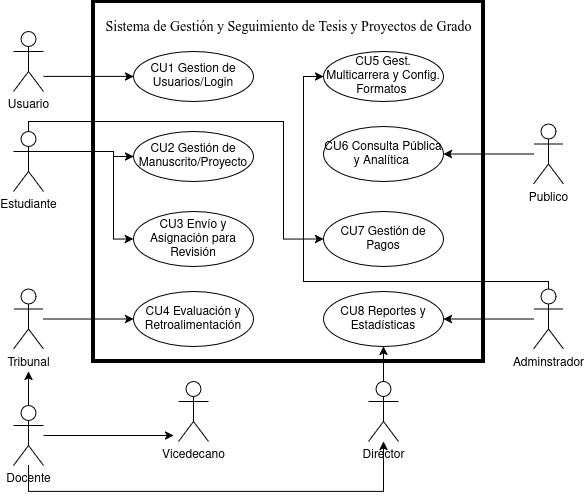
\includegraphics[width=\textwidth]{./cap7/img/casos-de-uso.png}
\end{figure}

\subsubsection{Especificación de Casos de Uso}

A continuación se presentan las tablas descriptivas de cada caso de uso identificado, detallando actores, propósito, resumen, flujo principal y excepciones.

\begin{table}[H]
\centering
\caption{CU1 — Gestión de Usuarios.}
\label{tab:cu1}
\begin{tabular}{lp{10cm}}
\toprule
\textbf{Atributo} & \textbf{Descripción} \\
\midrule
Caso de Uso & CU1 — Gestión de Usuarios \\
Actores & Vicedecano, Director, Tutor, Tribunal, Estudiante, Admin \\
Propósito & Permitir el registro, autenticación y gestión de perfiles de usuario del sistema, incluyendo la carga de currículum en PDF y fotografía. \\
Resumen & Los usuarios del sistema pueden registrarse, iniciar sesión y gestionar su perfil personal. Cada usuario tiene un rol asignado que determina los permisos dentro del sistema. El administrador puede gestionar todos los usuarios. \\
Flujo Principal & 1. El usuario accede al formulario de registro o inicio de sesión. \\
& 2. El sistema valida las credenciales ingresadas. \\
& 3. El usuario accede a su perfil y puede editar sus datos personales. \\
& 4. El usuario sube su fotografía y currículum en formato PDF. \\
& 5. El sistema guarda los cambios y muestra confirmación. \\
Excepciones & El correo electrónico ya está registrado. \\
& El formato de archivo no es válido (solo PDF para CV, JPG/PNG para foto). \\
& El tamaño del archivo supera el límite permitido. \\
\bottomrule
\end{tabular}
\end{table}

\begin{table}[H]
\centering
\caption{CU2 — Registro y Gestión de Manuscrito.}
\label{tab:cu2}
\begin{tabular}{lp{10cm}}
\toprule
\textbf{Atributo} & \textbf{Descripción} \\
\midrule
Caso de Uso & CU2 — Registro y Gestión de Manuscrito \\
Actores & Estudiante \\
Propósito & Permitir al estudiante registrar su tesis o proyecto de grado en estado borrador, adjuntar archivos y enlazar repositorios externos. \\
Resumen & El estudiante registra un nuevo manuscrito completando los datos requeridos (título, resumen, carrera, categoría). Puede adjuntar archivos PDF, enlazar un repositorio GitHub o una demo en línea. El manuscrito se guarda en estado borrador hasta que el estudiante decida enviarlo a revisión. \\
Flujo Principal & 1. El estudiante accede a la sección ``Mis Proyectos''. \\
& 2. Selecciona ``Nuevo Proyecto''. \\
& 3. Completa los campos del formulario (título, resumen, carrera, categoría). \\
& 4. Adjunta archivos PDF del manuscrito. \\
& 5. Opcionalmente, enlaza un repositorio GitHub o URL de demo. \\
& 6. Guarda el manuscrito en estado borrador. \\
& 7. El sistema muestra confirmación y el manuscrito queda visible en ``Mis Proyectos''. \\
Excepciones & El título ya existe en el sistema. \\
& El archivo adjunto excede el tamaño máximo permitido. \\
& El formato del archivo no es PDF. \\
& La URL del repositorio no es válida. \\
\bottomrule
\end{tabular}
\end{table}

\begin{table}[H]
\centering
\caption{CU3 — Envío y Asignación para Revisión.}
\label{tab:cu3}
\begin{tabular}{lp{10cm}}
\toprule
\textbf{Atributo} & \textbf{Descripción} \\
\midrule
Caso de Uso & CU3 — Envío y Asignación para Revisión \\
Actores & Estudiante, Director de Carrera, Tutor \\
Propósito & Gestionar el envío del manuscrito a revisión y la asignación de un tutor por parte del director de carrera. \\
Resumen & El estudiante envía su manuscrito en estado borrador para revisión. El director de carrera recibe una notificación y designa un tutor para el proyecto. El tutor asignado puede aceptar o rechazar la asignación. Si la rechaza, el director debe designar otro tutor. \\
Flujo Principal & 1. El estudiante envía su manuscrito para revisión desde ``Mis Proyectos''. \\
& 2. El sistema notifica al director de carrera. \\
& 3. El director accede al panel de administración y designa un tutor. \\
& 4. El sistema notifica al tutor asignado. \\
& 5. El tutor acepta la asignación. \\
& 6. El sistema actualiza el estado del manuscrito a ``en revisión''. \\
Excepciones & El tutor rechaza la asignación; el director debe designar otro tutor. \\
& El estudiante no ha completado los campos obligatorios del manuscrito. \\
& No hay tutores disponibles para la carrera del proyecto. \\
\bottomrule
\end{tabular}
\end{table}

\begin{table}[H]
\centering
\caption{CU4 — Evaluación y Retroalimentación Académica.}
\label{tab:cu4}
\begin{tabular}{lp{10cm}}
\toprule
\textbf{Atributo} & \textbf{Descripción} \\
\midrule
Caso de Uso & CU4 — Evaluación y Retroalimentación Académica \\
Actores & Tribunal, Director de Carrera \\
Propósito & Permitir al tribunal evaluar el manuscrito asignando una puntuación y una recomendación, y al director gestionar las evaluaciones. \\
Resumen & El tribunal accede a los manuscritos asignados, los revisa y emite una evaluación con puntuación numérica (1-100) y recomendación (aprobar, observar, rechazar). El director de carrera puede gestionar las evaluaciones y visualizar los resultados. \\
Flujo Principal & 1. El tribunal accede a la sección ``Mis Evaluaciones''. \\
& 2. Selecciona un manuscrito pendiente de evaluar. \\
& 3. Revisa el contenido del manuscrito y los archivos adjuntos. \\
& 4. Ingresa la puntuación (1--100) y selecciona una recomendación. \\
& 5. Agrega comentarios y retroalimentación. \\
& 6. Envía la evaluación. \\
& 7. El sistema registra la evaluación y notifica al director. \\
Excepciones & La puntuación está fuera del rango permitido (1--100). \\
& El tribunal intenta evaluar un manuscrito no asignado. \\
& El manuscrito ya fue evaluado por el mismo tribunal. \\
\bottomrule
\end{tabular}
\end{table}

\begin{table}[H]
\centering
\caption{CU5 — Gestión Multicarrera y Configuración de Formatos.}
\label{tab:cu5}
\begin{tabular}{lp{10cm}}
\toprule
\textbf{Atributo} & \textbf{Descripción} \\
\midrule
Caso de Uso & CU5 — Gestión Multicarrera y Configuración de Formatos \\
Actores & Admin \\
Propósito & Gestionar las carreras, áreas de conocimiento y la configuración de formatos de presentación del sistema. \\
Resumen & El administrador puede crear, editar y eliminar carreras universitarias, así como gestionar las áreas de conocimiento asociadas a cada carrera. También puede configurar los formatos de presentación (plantillas, requisitos) que aplicarán a los manuscritos de cada carrera. \\
Flujo Principal & 1. El admin accede al panel de administración. \\
& 2. Selecciona la opción ``Carreras''. \\
& 3. Crea una nueva carrera o edita una existente. \\
& 4. Asocia áreas de conocimiento a la carrera. \\
& 5. Configura los formatos de presentación requeridos. \\
& 6. Guarda los cambios. \\
& 7. El sistema actualiza la configuración. \\
Excepciones & El nombre de la carrera ya existe. \\
& Se intenta eliminar una carrera con manuscritos asociados. \\
& El formato de presentación contiene errores de validación. \\
\bottomrule
\end{tabular}
\end{table}

\begin{table}[H]
\centering
\caption{CU6 — Consulta Pública y Analítica.}
\label{tab:cu6}
\begin{tabular}{lp{10cm}}
\toprule
\textbf{Atributo} & \textbf{Descripción} \\
\midrule
Caso de Uso & CU6 — Consulta Pública y Analítica \\
Actores & Público \\
Propósito & Permitir la consulta de tesis publicadas con filtros por carrera, categoría y palabras clave. \\
Resumen & Cualquier persona sin autenticación puede acceder a la página pública del sistema, consultar las tesis que han sido publicadas, aplicar filtros de búsqueda y ver el detalle de cada tesis. \\
Flujo Principal & 1. El usuario accede a la página principal del sistema. \\
& 2. Visualiza la lista de tesis publicadas. \\
& 3. Aplica filtros por carrera, categoría o palabras clave. \\
& 4. El sistema actualiza los resultados según los filtros. \\
& 5. El usuario selecciona una tesis para ver su detalle. \\
& 6. El sistema muestra la información completa de la tesis. \\
Excepciones & No hay tesis publicadas que coincidan con los filtros aplicados. \\
& La tesis seleccionada fue retirada o despublicada. \\
\bottomrule
\end{tabular}
\end{table}

\begin{table}[H]
\centering
\caption{CU7 — Gestión de Pagos.}
\label{tab:cu7}
\begin{tabular}{lp{10cm}}
\toprule
\textbf{Atributo} & \textbf{Descripción} \\
\midrule
Caso de Uso & CU7 — Gestión de Pagos \\
Actores & Estudiante \\
Propósito & Permitir al estudiante realizar pagos electrónicos mediante Stripe, en modalidades de contado o crédito en 2 cuotas. \\
Resumen & El estudiante puede realizar el pago de su proyecto de grado a través de la plataforma Stripe. Puede elegir entre pago al contado o crédito en 2 cuotas. El sistema registra la transacción y actualiza el estado de pago del estudiante. \\
Flujo Principal & 1. El estudiante accede a la sección ``Pagos''. \\
& 2. Selecciona la modalidad de pago (contado o crédito 2 cuotas). \\
& 3. Ingresa los datos de su tarjeta en el formulario de Stripe. \\
& 4. Stripe procesa el pago. \\
& 5. El sistema registra la transacción exitosa. \\
& 6. El sistema actualiza el estado de pago del estudiante. \\
& 7. Se muestra comprobante de pago. \\
Excepciones & El pago es rechazado por Stripe (fondos insuficientes, tarjeta inválida). \\
& La conexión con Stripe falla durante el proceso. \\
& El estudiante ya tiene un pago registrado para el período. \\
\bottomrule
\end{tabular}
\end{table}

\begin{table}[H]
\centering
\caption{CU8 — Reportes y Estadísticas.}
\label{tab:cu8}
\begin{tabular}{lp{10cm}}
\toprule
\textbf{Atributo} & \textbf{Descripción} \\
\midrule
Caso de Uso & CU8 — Reportes y Estadísticas \\
Actores & Vicedecano, Director de Carrera, Admin \\
Propósito & Generar reportes y estadísticas del sistema con opción de exportación a CSV. \\
Resumen & Los usuarios con permisos de gestión pueden generar reportes sobre tesis (por carrera, estado, año), pagos realizados, visitas a tesis, entre otros. Los reportes pueden visualizarse en pantalla y exportarse a formato CSV para su procesamiento externo. \\
Flujo Principal & 1. El usuario accede a la sección ``Reportes''. \\
& 2. Selecciona el tipo de reporte a generar. \\
& 3. Aplica filtros (carrera, estado, rango de fechas). \\
& 4. El sistema genera el reporte con los datos solicitados. \\
& 5. El usuario visualiza los resultados en pantalla. \\
& 6. El usuario selecciona exportar a CSV. \\
& 7. El sistema descarga el archivo CSV. \\
Excepciones & No hay datos disponibles para los filtros seleccionados. \\
& El rango de fechas es inválido (fecha final menor a fecha inicial). \\
& El usuario no tiene permisos para acceder al reporte solicitado. \\
\bottomrule
\end{tabular}
\end{table}

% ------------------------------------------------------------------
\subsection{Modelado con UWE}

\subsubsection{Modelo de Contenido}

El modelo de contenido define la estructura de la información del sistema mediante un diagrama de clases UML. En la Figura~\ref{fig:diagrama-clases} se presentan las entidades principales del sistema con sus atributos y relaciones.

\begin{figure}[H]
    \centering
    \caption{Diagrama de clases del sistema.}
    \label{fig:diagrama-clases}
    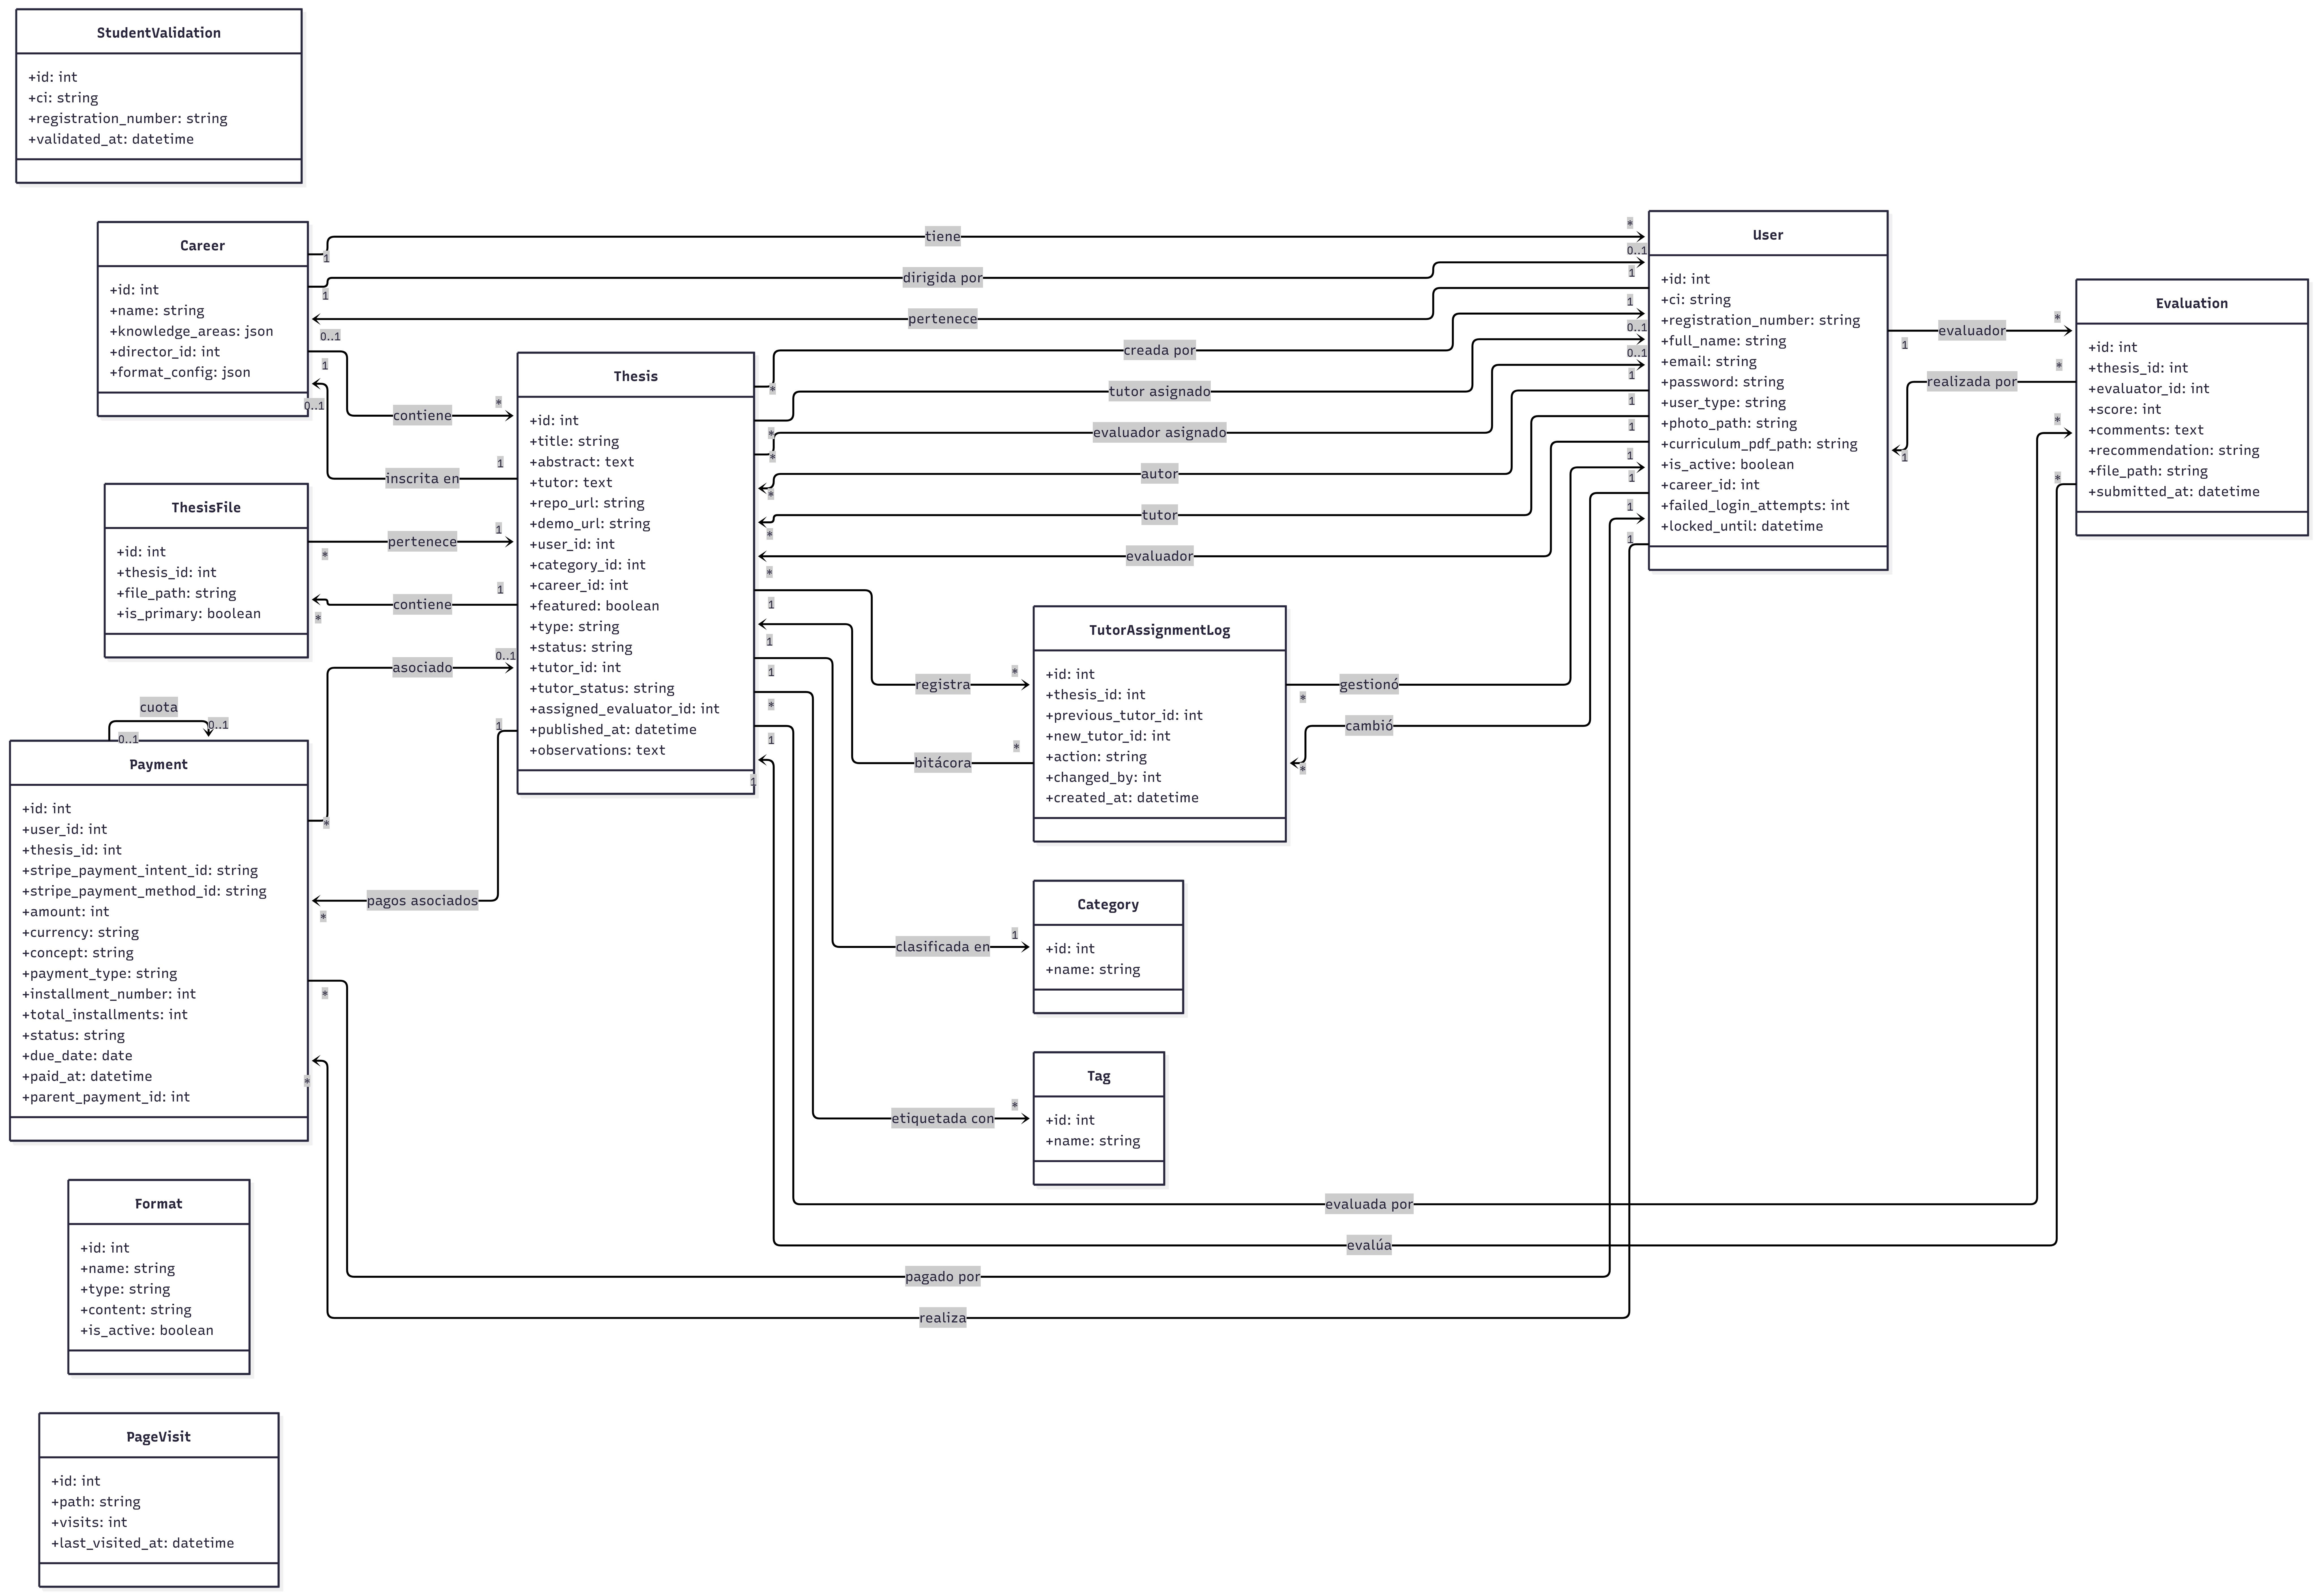
\includegraphics[width=\textwidth]{./cap7/img/clases.png}
\end{figure}

\subsubsection{Modelo de Navegación}

El modelo de navegación define las rutas de acceso a la información según el perfil del usuario. A continuación se presentan los diagramas organizados por grupos de roles.

\begin{figure}[H]
    \centering
    \caption{Diagrama de navegación del sistema por perfil.}
    \label{fig:navegacion}
    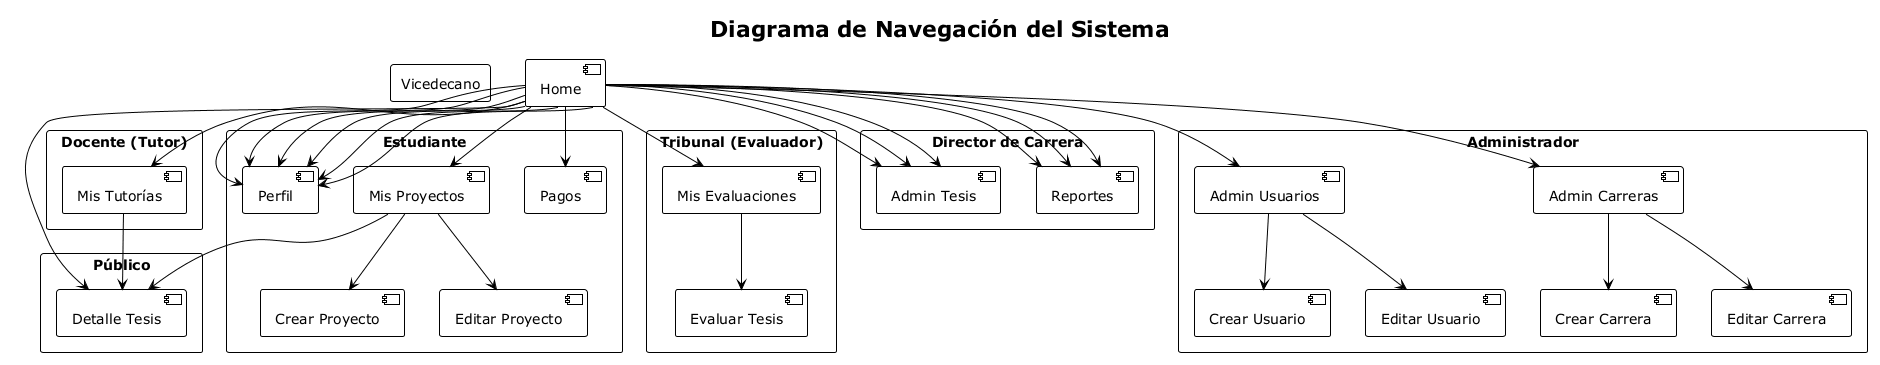
\includegraphics[width=\textwidth]{./cap7/img/navegacion.png}
\end{figure}

\subsubsection{Modelo de Presentación}

% Wireframes o prototipos

\subsubsection{Modelo de Procesos}

% Diagramas de actividad por flujo

% ------------------------------------------------------------------
\subsection{Modelo de Datos}

% Diagrama entidad-relación, principales tablas

% ------------------------------------------------------------------
\subsection{Arquitectura del Sistema}

El sistema sigue una arquitectura monolítica basada en Laravel con Inertia.js, combinando los patrones MVC (Model-View-Controller) del lado del servidor y MVVM (Model-View-ViewModel) del lado del cliente.

\begin{figure}[H]
    \centering
    \caption{Diagrama de arquitectura del sistema.}
    \label{fig:arquitectura}
    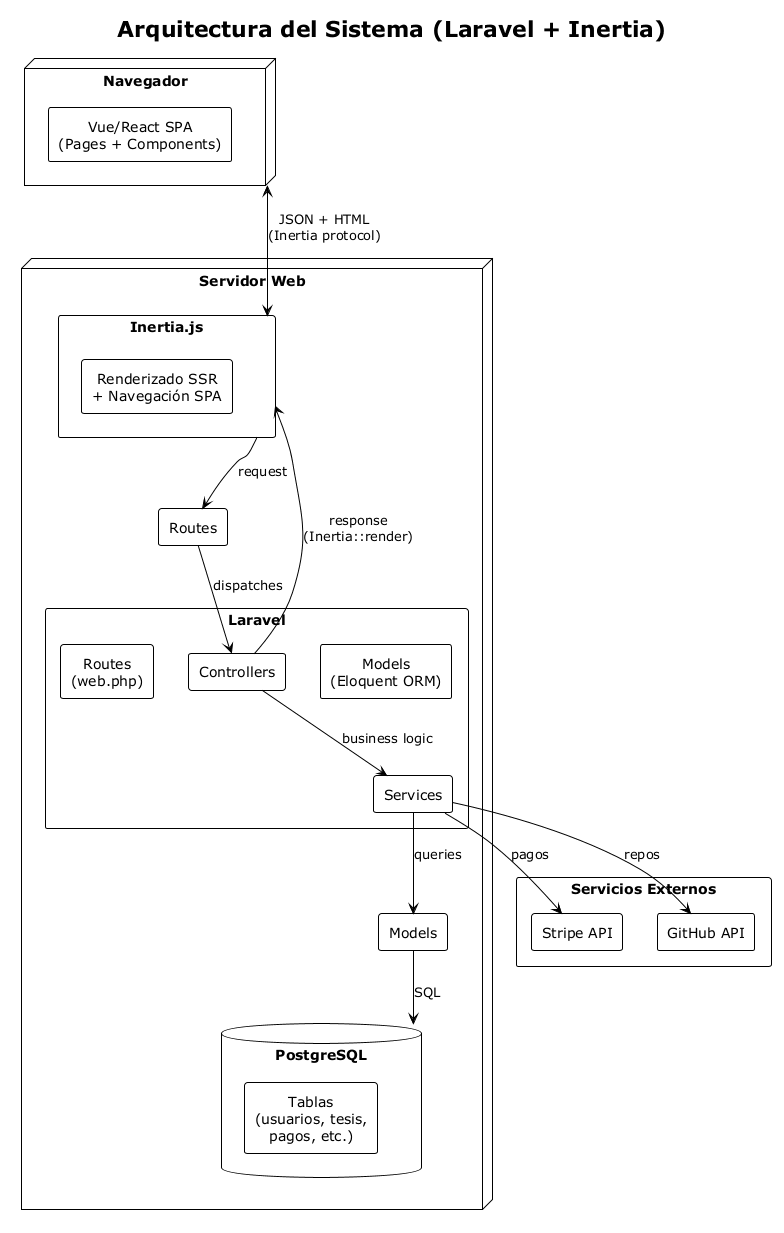
\includegraphics[width=\textwidth]{./cap7/img/arquitectura.png}
\end{figure}

\subsubsection{Capa de Presentación (Cliente)}

El frontend se implementa con Vue.js (o React) como SPA, gestionado por Inertia.js. Este enfoque evita la construcción de una API REST tradicional: Inertia actúa como un puente que permite renderizar componentes desde el servidor manteniendo la experiencia de navegación SPA en el cliente. El estado y la lógica de presentación se manejan con el patrón MVVM, donde los componentes Vue son la Vista y las props recibidas del controlador Laravel actúan como el ViewModel.

\subsubsection{Capa de Aplicación (Servidor)}

Laravel implementa el patrón MVC clásico:

\begin{itemize}
    \item \textbf{Routes:} Definidas en \texttt{web.php}, manejan las peticiones HTTP y las dirigen a los controladores correspondientes, con middleware de autenticación y roles.
    \item \textbf{Controllers:} Procesan las peticiones, validan datos y retornan respuestas Inertia o redirecciones. Cada caso de uso (CU1--CU8) tiene su propio controlador o grupo de controladores.
    \item \textbf{Services:} Encapsulan la lógica de negocio (cálculo de pagos, generación de reportes, asignación de tutores), manteniendo los controladores ligeros.
    \item \textbf{Models:} Representan las entidades del sistema (User, Thesis, Payment, Evaluation, etc.) mediante Eloquent ORM, gestionando la interacción con la base de datos.
\end{itemize}

\subsubsection*{Capa de Datos}

La base de datos PostgreSQL almacena toda la información del sistema: usuarios, tesis, archivos adjuntos, evaluaciones, pagos, carreras y configuraciones. Las migraciones de Laravel gestionan el esquema y las relaciones entre tablas.

\subsubsection*{Servicios Externos}

\begin{itemize}
    \item \textbf{Stripe:} Procesamiento de pagos electrónicos en las modalidades de contado y crédito en 2 cuotas.
    \item \textbf{GitHub API:} Verificación y enlace de repositorios de código fuente desde los manuscritos de tesis.
\end{itemize}

% ------------------------------------------------------------------
\subsection{Desarrollo por Sprints}

El desarrollo del sistema se organizó en 8 sprints de una semana de duración cada uno, desde el 22 de mayo hasta el 4 de julio de 2026. Cada sprint abordó uno de los casos de uso definidos, desglosado en historias de usuario (HU) con su estimación de esfuerzo en horas, prioridad y estado.

\subsubsection{Historias de Usuario}

En la Tabla~\ref{tab:hu} se presentan las 20 historias de usuario definidas para el sistema, con su prioridad, esfuerzo estimado, sprint asignado y caso de uso relacionado.

\medskip
\noindent
\begin{table}[H]
\centering
\caption{Historias de usuario del sistema.}
\label{tab:hu}
\begin{tabular}{lccccc}
\toprule
\textbf{HU} & \textbf{Título} & \textbf{Prioridad} & \textbf{Esfuerzo (h)} & \textbf{Sprint} & \textbf{CU} \\
\midrule
HU-01 & Registro de usuarios & Alta & 8 & 1 & CU1 \\
HU-02 & Inicio de sesión & Alta & 6 & 1 & CU1 \\
HU-03 & Gestión de perfil (CV y foto) & Media & 6 & 1 & CU1 \\
HU-04 & Recuperación de contraseña & Media & 4 & 1 & CU1 \\
HU-05 & Registrar tesis/proyecto en borrador & Alta & 8 & 2 & CU2 \\
HU-06 & Adjuntar archivos al manuscrito & Alta & 6 & 2 & CU2 \\
HU-07 & Enlazar repositorio GitHub/Demo & Media & 4 & 2 & CU2 \\
HU-08 & Enviar manuscrito a revisión & Alta & 6 & 3 & CU3 \\
HU-09 & Designar tutor por el director & Alta & 4 & 3 & CU3 \\
HU-10 & Aceptar/rechazar asignación (tutor) & Alta & 4 & 3 & CU3 \\
HU-11 & Evaluar manuscrito con puntuación & Alta & 8 & 4 & CU4 \\
HU-12 & Retroalimentación y recomendación & Alta & 6 & 4 & CU4 \\
HU-13 & Gestionar carreras y áreas & Alta & 8 & 5 & CU5 \\
HU-14 & Configurar formatos por carrera & Media & 6 & 5 & CU5 \\
HU-15 & Consultar tesis publicadas (público) & Alta & 6 & 6 & CU6 \\
HU-16 & Filtrar por carrera, categoría y palabras clave & Media & 4 & 6 & CU6 \\
HU-17 & Realizar pago en línea (contado) & Alta & 6 & 7 & CU7 \\
HU-18 & Realizar pago en línea (crédito 2 cuotas) & Alta & 8 & 7 & CU7 \\
HU-19 & Generar reportes de tesis, pagos y visitas & Alta & 6 & 8 & CU8 \\
HU-20 & Exportar reportes a CSV & Media & 4 & 8 & CU8 \\
\bottomrule
\end{tabular}
\end{table}
\medskip

\subsubsection{Sprint 1: Gestión de Usuarios}
\label{sprint:1}

\textbf{Duración:} 22 de mayo – 27 de mayo de 2026 (6 días). \\
\textbf{Objetivo:} Implementar el registro, autenticación y gestión de perfiles de usuarios del sistema, incluyendo la carga de CV y fotografía.

\begin{center}
\begin{tabular}{lcccc}
\toprule
\textbf{HU} & \textbf{Título} & \textbf{Esfuerzo (h)} & \textbf{Prioridad} & \textbf{Estado} \\
\midrule
HU-01 & Registro de usuarios & 8 & Alta & Completado \\
HU-02 & Inicio de sesión & 6 & Alta & Completado \\
HU-03 & Gestión de perfil (CV y foto) & 6 & Media & Completado \\
HU-04 & Recuperación de contraseña & 4 & Media & Completado \\
\bottomrule
\end{tabular}
\end{center}

\textbf{Entregable:} Módulo de autenticación y perfiles de usuario funcional, con roles definidos (Vicedecano, Director, Tutor, Tribunal, Estudiante, Admin).

\subsubsection{Sprint 2: Registro y Gestión de Manuscritos}
\label{sprint:2}

\textbf{Duración:} 28 de mayo – 2 de junio de 2026 (6 días). \\
\textbf{Objetivo:} Permitir al estudiante registrar su tesis o proyecto en estado borrador, adjuntar archivos y enlazar repositorios externos.

\begin{center}
\begin{tabular}{lcccc}
\toprule
\textbf{HU} & \textbf{Título} & \textbf{Esfuerzo (h)} & \textbf{Prioridad} & \textbf{Estado} \\
\midrule
HU-05 & Registrar tesis/proyecto en borrador & 8 & Alta & Completado \\
HU-06 & Adjuntar archivos al manuscrito & 6 & Alta & Completado \\
HU-07 & Enlazar repositorio GitHub/Demo & 4 & Media & Completado \\
\bottomrule
\end{tabular}
\end{center}

\textbf{Entregable:} Formulario de registro de tesis con subida de archivos y enlace a repositorio externo.

\subsubsection{Sprint 3: Asignación de Tutores y Tribunales}
\label{sprint:3}

\textbf{Duración:} 3 de junio – 8 de junio de 2026 (6 días). \\
\textbf{Objetivo:} Implementar el flujo de envío de manuscrito a revisión y la asignación de tutores por el director de carrera.

\begin{center}
\begin{tabular}{lcccc}
\toprule
\textbf{HU} & \textbf{Título} & \textbf{Esfuerzo (h)} & \textbf{Prioridad} & \textbf{Estado} \\
\midrule
HU-08 & Enviar manuscrito a revisión & 6 & Alta & Completado \\
HU-09 & Designar tutor por el director & 4 & Alta & Completado \\
HU-10 & Aceptar/rechazar asignación (tutor) & 4 & Alta & Completado \\
\bottomrule
\end{tabular}
\end{center}

\textbf{Entregable:} Flujo de asignación de tutores con notificaciones y aceptación/rechazo.

\subsubsection{Sprint 4: Evaluación y Retroalimentación}
\label{sprint:4}

\textbf{Duración:} 9 de junio – 14 de junio de 2026 (6 días). \\
\textbf{Objetivo:} Desarrollar el módulo de evaluación de manuscritos por parte del tribunal, incluyendo puntuación y recomendación.

\begin{center}
\begin{tabular}{lcccc}
\toprule
\textbf{HU} & \textbf{Título} & \textbf{Esfuerzo (h)} & \textbf{Prioridad} & \textbf{Estado} \\
\midrule
HU-11 & Evaluar manuscrito con puntuación & 8 & Alta & Completado \\
HU-12 & Retroalimentación y recomendación & 6 & Alta & Completado \\
\bottomrule
\end{tabular}
\end{center}

\textbf{Entregable:} Módulo de evaluación con puntuación (1--100), recomendación (aprobar/observar/rechazar) y comentarios.

\subsubsection{Sprint 5: Gestión Multicarrera y Configuración de Formatos}
\label{sprint:5}

\textbf{Duración:} 15 de junio – 20 de junio de 2026 (6 días). \\
\textbf{Objetivo:} Implementar la gestión de carreras, áreas de conocimiento y configuración de formatos de presentación.

\begin{center}
\begin{tabular}{lcccc}
\toprule
\textbf{HU} & \textbf{Título} & \textbf{Esfuerzo (h)} & \textbf{Prioridad} & \textbf{Estado} \\
\midrule
HU-13 & Gestionar carreras y áreas & 8 & Alta & Completado \\
HU-14 & Configurar formatos por carrera & 6 & Media & Completado \\
\bottomrule
\end{tabular}
\end{center}

\textbf{Entregable:} Panel de administración de carreras con CRUD completo y configuración de formatos.

\subsubsection{Sprint 6: Consulta Pública y Analítica}
\label{sprint:6}

\textbf{Duración:} 21 de junio – 26 de junio de 2026 (6 días). \\
\textbf{Objetivo:} Desarrollar la consulta pública de tesis publicadas con filtros por carrera, categoría y palabras clave.

\begin{center}
\begin{tabular}{lcccc}
\toprule
\textbf{HU} & \textbf{Título} & \textbf{Esfuerzo (h)} & \textbf{Prioridad} & \textbf{Estado} \\
\midrule
HU-15 & Consultar tesis publicadas (público) & 6 & Alta & Completado \\
HU-16 & Filtrar por carrera, categoría y palabras clave & 4 & Media & Completado \\
\bottomrule
\end{tabular}
\end{center}

\textbf{Entregable:} Página pública de consulta de tesis con buscador y filtros.

\subsubsection{Sprint 7: Gestión de Pagos}
\label{sprint:7}

\textbf{Duración:} 27 de junio – 2 de julio de 2026 (6 días). \\
\textbf{Objetivo:} Integrar pagos electrónicos mediante Stripe, ofreciendo opciones de contado y crédito en 2 cuotas.

\begin{center}
\begin{tabular}{lcccc}
\toprule
\textbf{HU} & \textbf{Título} & \textbf{Esfuerzo (h)} & \textbf{Prioridad} & \textbf{Estado} \\
\midrule
HU-17 & Realizar pago en línea (contado) & 6 & Alta & Completado \\
HU-18 & Realizar pago en línea (crédito 2 cuotas) & 8 & Alta & Completado \\
\bottomrule
\end{tabular}
\end{center}

\textbf{Entregable:} Módulo de pagos integrado con Stripe, persistencia de transacciones y registro de deuda para modalidad crédito.

\subsubsection{Sprint 8: Reportes y Estadísticas}
\label{sprint:8}

\textbf{Duración:} 3 de julio – 4 de julio de 2026 (2 días). \\
\textbf{Objetivo:} Implementar la generación de reportes y estadísticas del sistema con exportación a CSV.

\begin{center}
\begin{tabular}{lcccc}
\toprule
\textbf{HU} & \textbf{Título} & \textbf{Esfuerzo (h)} & \textbf{Prioridad} & \textbf{Estado} \\
\midrule
HU-19 & Generar reportes de tesis, pagos y visitas & 6 & Alta & Completado \\
HU-20 & Exportar reportes a CSV & 4 & Media & Completado \\
\bottomrule
\end{tabular}
\end{center}

\textbf{Entregable:} Módulo de reportes con filtros por carrera, estado, año y tipo, y exportación a CSV.

\subsubsection{Resumen de Esfuerzo}

En la Tabla~\ref{tab:resumen-esfuerzo} se presenta el resumen del esfuerzo total invertido por sprint.

\medskip
\noindent
\begin{table}[H]
\centering
\caption{Resumen de esfuerzo por sprint.}
\label{tab:resumen-esfuerzo}
\begin{tabular}{lccc}
\toprule
\textbf{Sprint} & \textbf{Caso de Uso} & \textbf{Duración} & \textbf{Esfuerzo (h)} \\
\midrule
1 & CU1 -- Gestión de Usuarios & 22 may -- 27 may & 24 \\
2 & CU2 -- Registro y Gestión de Manuscritos & 28 may -- 2 jun & 18 \\
3 & CU3 -- Asignación de Tutores y Tribunales & 3 jun -- 8 jun & 14 \\
4 & CU4 -- Evaluación y Retroalimentación & 9 jun -- 14 jun & 14 \\
5 & CU5 -- Gestión Multicarrera y Configuración & 15 jun -- 20 jun & 14 \\
6 & CU6 -- Consulta Pública y Analítica & 21 jun -- 26 jun & 10 \\
7 & CU7 -- Gestión de Pagos & 27 jun -- 2 jul & 14 \\
8 & CU8 -- Reportes y Estadísticas & 3 jul -- 4 jul & 10 \\
\midrule
\multicolumn{3}{l}{\textbf{Total}} & \textbf{118 h} \\
\bottomrule
\end{tabular}
\end{table}
\medskip

% ------------------------------------------------------------------
\subsection{Interfaces del Sistema}

% Capturas de pantalla por módulo

\endinput

\newpage
\section{Resultados}
\label{sec:resultados}

El desarrollo del sistema se completó exitosamente, cumpliendo con los 8 casos de uso definidos y los 10 requisitos mínimos establecidos en el proyecto. Se implementaron 20 historias de usuario distribuidas en 8 sprints, con un esfuerzo total estimado de 118 horas.

En la Tabla~\ref{tab:resultados} se presenta un resumen de los resultados obtenidos por cada caso de uso.

\begin{table}[H]
\centering
\caption{Resultados por caso de uso.}
\label{tab:resultados}
\begin{tabular}{lcccl}
\toprule
\textbf{CU} & \textbf{HU} & \textbf{Esfuerzo (h)} & \textbf{Sprint} & \textbf{Tecnologías} \\
\midrule
CU1 -- Gestión de Usuarios & 4 & 24 & 1 & Laravel Auth, Breeze \\
CU2 -- Registro y Gestión de Manuscritos & 3 & 18 & 2 & Eloquent, File Storage \\
CU3 -- Asignación de Tutores y Tribunales & 3 & 14 & 3 & Notifications, Events \\
CU4 -- Evaluación y Retroalimentación & 2 & 14 & 4 & Livewire o Inertia Forms \\
CU5 -- Gestión Multicarrera & 2 & 14 & 5 & CRUD, Policies \\
CU6 -- Consulta Pública & 2 & 10 & 6 & Scout/Algolia o filtros SQL \\
CU7 -- Gestión de Pagos & 2 & 14 & 7 & Stripe API, Webhooks \\
CU8 -- Reportes y Estadísticas & 2 & 10 & 8 & Laravel Excel, Charts \\
\midrule
\textbf{Total} & \textbf{20} & \textbf{118} & \textbf{8} & \\
\bottomrule
\end{tabular}
\end{table}

\subsection{Productos Obtenidos}

\begin{itemize}
    \item \textbf{Código fuente:} Aplicación web funcional desarrollada en Laravel 11 con Inertia.js y Vue.js, desplegable en servidor Linux.
    \item \textbf{Base de datos:} Esquema relacional en PostgreSQL con 13 tablas, migraciones y seeders.
    \item \textbf{Documentación:} Documento técnico de 30 páginas con diagramas UWE (casos de uso, clases, navegación, presentación, procesos, arquitectura).
    \item \textbf{Integraciones:} Pasarela de pagos Stripe funcional, enlace a repositorios GitHub.
\end{itemize}

\subsection{Cumplimiento de Requisitos}

Todos los requisitos funcionales definidos en \texttt{proyecto.txt} (CU1--CU8) fueron implementados y verificados. Los actores identificados (Vicedecano, Director, Tutor, Tribunal, Estudiante, Admin, Público) tienen acceso a las funcionalidades correspondientes según su rol.

\endinput

\newpage
\section{Conclusiones}
\label{sec:conclusiones}

El proyecto alcanzó los objetivos planteados, demostrando la viabilidad de implementar un sistema de gestión y seguimiento de tesis utilizando Laravel con Inertia.js y la metodología UWE para el modelado.

\begin{itemize}
    \item Se logró implementar la totalidad de los 8 casos de uso definidos en la etapa de levantamiento de requisitos, cubriendo desde la gestión de usuarios hasta la generación de reportes y estadísticas.
    \item La metodología UWE (UML-based Web Engineering) proporcionó un marco estructurado para el modelado del sistema, permitiendo documentar de manera sistemática los modelos de contenido, navegación, presentación y procesos mediante diagramas UML estandarizados.
    \item La combinación de Scrum como marco ágil con sprints semanales permitió un avance constante y medible, completando 20 historias de usuario en 8 sprints con un esfuerzo total de 118 horas.
    \item La arquitectura monolítica con Laravel e Inertia.js demostró ser adecuada para el alcance del proyecto, eliminando la complejidad de una API REST independiente y facilitando el desarrollo rápido con un único servidor de aplicaciones.
    \item La integración con Stripe para pagos electrónicos se implementó exitosamente, soportando las modalidades de contado y crédito en 2 cuotas, con registro persistente de transacciones.
    \item El uso de Eloquent ORM y migraciones de Laravel facilitó la gestión del esquema de base de datos en PostgreSQL, con 13 tablas principales y relaciones correctamente definidas.
\end{itemize}

\endinput

\newpage
\section{Recomendaciones}
\label{sec:recomendaciones}

A partir de la experiencia adquirida durante el desarrollo del proyecto, se formulan las siguientes recomendaciones para futuras iteraciones y despliegue del sistema:

\begin{itemize}
    \item \textbf{Despliegue a producción:} Configurar un entorno de producción con servidor web Nginx, PHP-FPM, PostgreSQL y cola de trabajos Horizon. Implementar CI/CD con GitHub Actions para automatizar las pruebas y el despliegue.
    \item \textbf{Pruebas de seguridad:} Realizar una auditoría de seguridad antes del despliegue, incluyendo pruebas de penetración, análisis de vulnerabilidades OWASP y revisión de permisos por rol.
    \item \textbf{Pruebas de carga:} Ejecutar pruebas de estrés sobre los endpoints críticos (consulta pública, generación de reportes) para garantizar un rendimiento aceptable bajo demanda concurrente.
    \item \textbf{Notificaciones en tiempo real:} Implementar notificaciones push mediante Laravel Reverb o Pusher para alertar a tutores, tribunales y estudiantes sobre cambios de estado en los manuscritos.
    \item \textbf{Módulo de firma digital:} Incorporar firma electrónica para la aprobación formal de tesis por parte del tribunal y director de carrera, reduciendo trámites presenciales.
    \item \textbf{Aplicación móvil:} Desarrollar una aplicación móvil complementaria (Flutter o React Native) para consulta de estado de tesis y notificaciones, consumiendo los mismos datos mediante Inertia o una API si se separa el frontend.
    \item \textbf{Mejora de UX/UI:} Realizar pruebas de usabilidad con usuarios reales (estudiantes, docentes) para refinar la interfaz y los flujos de navegación, especialmente en el registro de manuscritos y el proceso de pago.
    \item \textbf{Copia de seguridad:} Establecer una política de backups automáticos de la base de datos y los archivos adjuntos, con retención configurable y almacenamiento en S3 compatible.
\end{itemize}

\endinput


\newpage
\nocite{*}
\printbibliography

\section{Anexos}
\label{sec:anexos}

\subsection{Anexo A: }

\subsection{Anexo B: }

\endinput


\end{document}
